\documentclass[11pt,a4paper]{article}

\usepackage[margin=1in]{geometry}
\usepackage{mathptmx}
\usepackage{amsmath}
\usepackage{amssymb}
\usepackage{amsthm}
\usepackage{braket}
\usepackage{tikz}
\usepackage{quantikz}
\usepackage{enumitem}
\usepackage{hyperref}
\usepackage{xcolor}

\definecolor{circuitblue}{RGB}{40,80,160}

\hypersetup{
    colorlinks=true,
    linkcolor=circuitblue,
    urlcolor=circuitblue,
    citecolor=circuitblue
}

\theoremstyle{definition}
\newtheorem{definition}{Definition}[section]
\newtheorem{example}{Example}[section]

\theoremstyle{remark}
\newtheorem*{intuition}{Intuition}
\newtheorem*{keypoint}{Key Point}

\pagestyle{plain}

\setlength{\parindent}{0pt}
\setlength{\parskip}{6pt}

\begin{document}

\begin{center}
    {\LARGE \textbf{QAOA and Applications}}\\[8pt]
    {\large QML}\\[12pt]
    \hrule
\end{center}

\vspace{12pt}
\tableofcontents
\newpage

%% ========================================================
\section{Overview}
%% ========================================================

the quantum approximate optimization algorithm (QAOA) is one of the most important variational quantum algorithms. its designed for combinatorial optimization problems --- things like MaxCut, traveling salesman, portfolio optimization, scheduling. these problems r NP-hard classically, and while QAOA probably doesnt solve them in polynomial time, it might give better approximations than classical algorithms for certain instances.

QAOA is also important for QML bcs it shares the same variational framework as quantum classifiers. the circuit structure, parameter optimization, and trainability issues r all the same. understanding QAOA gives u a concrete example of how parameterized quantum circuits r used to solve real problems.

%% ========================================================
\section{Combinatorial Optimization}
%% ========================================================

\subsection{The Setup}

\begin{definition}
a \textbf{combinatorial optimization problem} asks: given a finite set of candidate solutions and an objective function, find the solution that maximizes (or minimizes) the objective.

formally: $\max_{z \in \{0,1\}^n} C(z)$ where $C$ is the cost function and $z$ is an $n$-bit binary string.
\end{definition}

\subsection{MaxCut}

\begin{definition}
given a graph $G = (V, E)$, find a partition of the vertices into two sets that maximizes the number of edges between the sets (edges that are ``cut'').

cost function:
\[
C(z) = \sum_{(i,j) \in E} \frac{1 - z_i z_j}{2}
\]
where $z_i \in \{-1, +1\}$ indicates which set vertex $i$ belongs to.
\end{definition}

\begin{center}
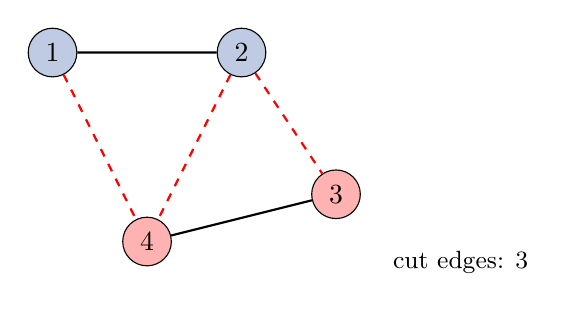
\begin{tikzpicture}[scale=1.2]
    % nodes
    \node[draw, circle, fill=circuitblue!30, minimum size=0.6cm] (1) at (0, 2) {1};
    \node[draw, circle, fill=circuitblue!30, minimum size=0.6cm] (2) at (2, 2) {2};
    \node[draw, circle, fill=red!30, minimum size=0.6cm] (3) at (3, 0.5) {3};
    \node[draw, circle, fill=red!30, minimum size=0.6cm] (4) at (1, 0) {4};

    % edges
    \draw[thick] (1) -- (2);
    \draw[thick, dashed, red] (1) -- (4);
    \draw[thick, dashed, red] (2) -- (3);
    \draw[thick, dashed, red] (2) -- (4);
    \draw[thick] (3) -- (4);

    \node[below right, font=\small] at (3.5, 0) {cut edges: 3};
\end{tikzpicture}
\end{center}

maxcut is NP-hard in general. the best known classical approximation algorithm (Goemans-Williamson, 1995) achieves a ratio of $\approx 0.878$, and improving this is a major open problem (assuming the unique games conjecture).

\subsection{Other Combinatorial Problems}

\begin{itemize}
    \item \textbf{traveling salesman problem (TSP)}: find the shortest route visiting all cities exactly once
    \item \textbf{graph coloring}: color vertices such that no two adjacent vertices have the same color, using minimum colors
    \item \textbf{portfolio optimization}: maximize return while minimizing risk, subject to constraints
    \item \textbf{job scheduling}: assign jobs to machines to minimize total completion time
\end{itemize}

all of these can be formulated as QUBO (quadratic unconstrained binary optimization) problems.

\subsection{QUBO Formulation}

\begin{definition}
a \textbf{QUBO} (quadratic unconstrained binary optimization) problem:
\[
\min_{x \in \{0,1\}^n} x^T Q x
\]
where $Q$ is an $n \times n$ upper triangular matrix encoding the objective function. diagonal elements encode linear terms, off-diagonal elements encode quadratic interactions.
\end{definition}

\begin{keypoint}
any QUBO can be mapped to an \textbf{Ising hamiltonian} by the substitution $x_i = (1 - z_i)/2$ where $z_i \in \{-1, +1\}$:
\[
H_C = \sum_{i} h_i Z_i + \sum_{i < j} J_{ij} Z_i Z_j + \text{const}
\]
this is a diagonal hamiltonian in the computational basis. its eigenvalues encode the cost function values. the ground state of $H_C$ is the optimal solution.
\end{keypoint}

\begin{example}
MaxCut on a triangle graph (3 vertices, 3 edges):

cost function: $C(z) = \frac{1}{2}(3 - z_1 z_2 - z_2 z_3 - z_1 z_3)$

ising hamiltonian:
\[
H_C = -\frac{1}{2}(Z_1 Z_2 + Z_2 Z_3 + Z_1 Z_3) + \frac{3}{2}I
\]

the ground state of $-H_C$ (or maximum of $H_C$) gives the optimal cut. by symmetry, the maximum cut is 2 (cut any 2 edges).
\end{example}

%% ========================================================
\section{The QAOA Algorithm}
%% ========================================================

\subsection{The Circuit}

QAOA was introduced by farhi, goldstone, and gutmann (2014). the algorithm uses a PQC with a specific alternating structure:

\begin{definition}
\textbf{QAOA} with $p$ layers:
\begin{enumerate}
    \item \textbf{initialize}: $\ket{+}^{\otimes n} = H^{\otimes n}\ket{0}^{\otimes n}$ (uniform superposition)
    \item \textbf{apply $p$ layers} of alternating unitaries:
    \[
    \ket{\gamma, \beta} = \underbrace{e^{-i\beta_p B} e^{-i\gamma_p C}}_{\text{layer } p} \cdots \underbrace{e^{-i\beta_1 B} e^{-i\gamma_1 C}}_{\text{layer } 1} \ket{+}^{\otimes n}
    \]
    \item \textbf{measure}: compute $\langle C \rangle = \bra{\gamma, \beta} C \ket{\gamma, \beta}$
    \item \textbf{optimize}: use a classical optimizer to find $\gamma^*, \beta^*$ that maximize $\langle C \rangle$
\end{enumerate}
\end{definition}

where:
\begin{itemize}
    \item $C = H_C$ is the \textbf{problem (cost) hamiltonian} --- diagonal in the computational basis, encodes the optimization objective
    \item $B = \sum_{i=1}^n X_i$ is the \textbf{mixer hamiltonian} --- creates transitions between computational basis states
    \item $\gamma = (\gamma_1, \ldots, \gamma_p)$ and $\beta = (\beta_1, \ldots, \beta_p)$ r the variational parameters ($2p$ total)
\end{itemize}

\subsection{QAOA Circuit Diagram}

for MaxCut on a 4-vertex graph with $p = 1$:

\begin{center}
\begin{quantikz}
\lstick{$\ket{0}$} & \gate{H} & \gate[2]{ZZ(\gamma_1)} & \qw & \qw & \gate{R_x(2\beta_1)} & \meter{} \\
\lstick{$\ket{0}$} & \gate{H} & & \gate[2]{ZZ(\gamma_1)} & \qw & \gate{R_x(2\beta_1)} & \meter{} \\
\lstick{$\ket{0}$} & \gate{H} & \qw & & \gate[2]{ZZ(\gamma_1)} & \gate{R_x(2\beta_1)} & \meter{} \\
\lstick{$\ket{0}$} & \gate{H} & \qw & \qw & & \gate{R_x(2\beta_1)} & \meter{}
\end{quantikz}
\end{center}

where $ZZ(\gamma) = e^{-i\gamma Z_i Z_j/2}$ is the $ZZ$-interaction gate for each edge $(i,j)$ in the graph.

\subsection{The Cost Unitary}

\[
e^{-i\gamma C} = \prod_{(i,j) \in E} e^{-i\gamma Z_i Z_j / 2}
\]

each $ZZ$-interaction can be decomposed into native gates:

\begin{center}
\begin{quantikz}
& \ctrl{1} & \qw & \ctrl{1} & \qw \\
& \targ{} & \gate{R_z(2\gamma)} & \targ{} & \qw
\end{quantikz}
\end{center}

this implements $e^{-i\gamma Z_i Z_j}$ (up to global phase) using two CNOTs and one $R_z$ gate.

\subsection{The Mixer Unitary}

\[
e^{-i\beta B} = e^{-i\beta \sum_j X_j} = \prod_j e^{-i\beta X_j} = \prod_j R_x(2\beta)
\]

the mixer is just individual $R_x$ rotations on each qubit --- easy to implement.

%% ========================================================
\section{Why QAOA Works}
%% ========================================================

\subsection{Connection to Adiabatic Quantum Computing}

\begin{intuition}
QAOA can be understood as a \textbf{trotterized version of adiabatic quantum computing}.

in adiabatic QC, u start with the ground state of an easy hamiltonian $B$ (which is $\ket{+}^{\otimes n}$ for $B = \sum X_i$) and slowly evolve to the ground state of the problem hamiltonian $C$. the adiabatic theorem says if u go slowly enough, u stay in the ground state throughout.

QAOA approximates this continuous evolution with $p$ discrete steps. as $p \to \infty$, QAOA can reproduce the adiabatic evolution exactly. for finite $p$, QAOA is a variational approximation --- the optimizer finds the best discrete schedule.
\end{intuition}

\begin{keypoint}
the relationship:
\begin{itemize}
    \item $p = 1$: very coarse approximation. can still beat random guessing but typically far from optimal.
    \item $p = O(\text{poly}(n))$: can approximate adiabatic evolution. in principle, can find the optimal solution.
    \item $p \to \infty$: converges to the exact solution (under mild conditions).
    \item in practice on NISQ hardware: $p \sim 1$--$10$ due to noise constraints.
\end{itemize}
\end{keypoint}

\subsection{QAOA Performance Guarantees}

\begin{keypoint}
for MaxCut on 3-regular graphs (every vertex has degree 3), farhi et al. showed that QAOA with $p = 1$ achieves an approximation ratio of at least $0.6924$ (i.e., cuts at least $69.24\%$ of the maximum number of cuttable edges).

compare to:
\begin{itemize}
    \item random assignment: $0.5$ (50\% of edges cut in expectation)
    \item greedy algorithm: can do better than random but no worst-case guarantee
    \item goemans-williamson SDP: $0.878$ ratio
    \item QAOA $p = 1$: $0.6924$
    \item QAOA with larger $p$: approaches $1.0$ as $p$ increases
\end{itemize}

so $p = 1$ QAOA doesnt beat goemans-williamson. but for larger $p$, QAOA might outperform classical algorithms for certain instances. this is an active research question.
\end{keypoint}

%% ========================================================
\section{Parameter Optimization in QAOA}
%% ========================================================

\subsection{The Optimization Landscape}

QAOA has $2p$ parameters: $\gamma_1, \ldots, \gamma_p, \beta_1, \ldots, \beta_p$.

for small $p$, the landscape is low-dimensional and can be explored relatively easily. for $p = 1$ (just 2 parameters), u can even plot the landscape:

\begin{center}
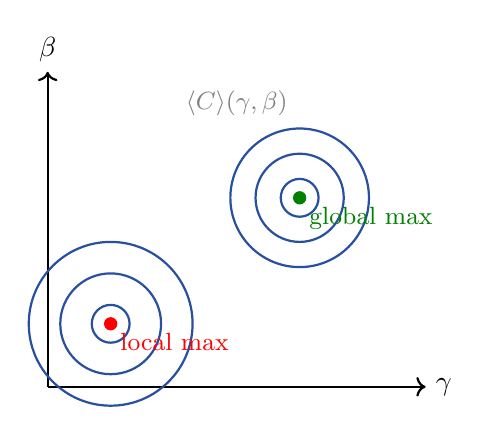
\begin{tikzpicture}[scale=0.8]
    \draw[->, thick] (0,0) -- (6,0) node[right] {$\gamma$};
    \draw[->, thick] (0,0) -- (0,5) node[above] {$\beta$};

    % contour-like shading
    \draw[circuitblue, thick] (1,1) circle (0.3);
    \draw[circuitblue, thick] (1,1) circle (0.8);
    \draw[circuitblue, thick] (1,1) circle (1.3);
    \draw[circuitblue, thick] (4,3) circle (0.3);
    \draw[circuitblue, thick] (4,3) circle (0.7);
    \draw[circuitblue, thick] (4,3) circle (1.1);

    \fill[red] (1,1) circle (3pt) node[below right, font=\small] {local max};
    \fill[green!50!black] (4,3) circle (3pt) node[below right, font=\small] {global max};

    \node[font=\small, gray] at (3,4.5) {$\langle C \rangle(\gamma, \beta)$};
\end{tikzpicture}
\end{center}

\subsection{Optimization Strategies}

\textbf{grid search} (for $p = 1$, 2): systematically evaluate $\langle C \rangle$ on a grid of $(\gamma, \beta)$ values. simple and works for low $p$.

\textbf{classical optimizers}: COBYLA, Nelder-Mead, L-BFGS-B for small $p$. gradient-based methods (using parameter shift rule) for larger $p$.

\textbf{parameter initialization}: random initialization can get stuck in local minima. strategies:
\begin{itemize}
    \item \textbf{linear ramp}: set $\gamma_k = k \gamma_{\max}/p$ and $\beta_k = (1 - k/p) \beta_{\max}$ (mimics adiabatic schedule)
    \item \textbf{INTERP}: optimize for $p$ layers, then interpolate to get initial parameters for $p+1$ layers (layer-by-layer growth)
    \item \textbf{transfer learning}: optimize on a small instance, transfer optimal angles to a larger instance of the same problem type
\end{itemize}

\begin{keypoint}
a nice property of QAOA: the optimal parameters for MaxCut often concentrate --- they tend to be similar across different graph instances of the same type and size. this means u can ``pre-train'' on small graphs and transfer the parameters.
\end{keypoint}

\subsection{Symmetries and Parameter Periodicity}

the QAOA cost function has symmetries that can be exploited:
\begin{itemize}
    \item $\gamma$ and $\beta$ r periodic: $\gamma \in [0, 2\pi)$, $\beta \in [0, \pi)$
    \item for MaxCut: the landscape has additional symmetries that reduce the search space
    \item these symmetries can be used to restrict the optimization domain
\end{itemize}

%% ========================================================
\section{QAOA Worked Example: MaxCut on a Triangle}
%% ========================================================

\begin{example}
MaxCut on a triangle graph (3 vertices, 3 edges) with $p = 1$.

\textbf{cost hamiltonian}:
\[
C = \frac{1}{2}(3I - Z_1 Z_2 - Z_2 Z_3 - Z_1 Z_3)
\]

\textbf{cost unitary}:
\[
e^{-i\gamma C} = e^{-i3\gamma/2} \cdot e^{i\gamma Z_1 Z_2/2} \cdot e^{i\gamma Z_2 Z_3/2} \cdot e^{i\gamma Z_1 Z_3/2}
\]

\textbf{mixer unitary}:
\[
e^{-i\beta B} = R_x(2\beta)_1 \otimes R_x(2\beta)_2 \otimes R_x(2\beta)_3
\]

\textbf{circuit}:
\begin{center}
\begin{quantikz}
\lstick{$\ket{0}$} & \gate{H} & \ctrl{1} & \qw & \ctrl{2} & \qw & \qw & \qw & \gate{R_x(2\beta)} & \meter{} \\
\lstick{$\ket{0}$} & \gate{H} & \targ{} & \gate{R_z(\gamma)} & \qw & \ctrl{1} & \qw & \qw & \gate{R_x(2\beta)} & \meter{} \\
\lstick{$\ket{0}$} & \gate{H} & \qw & \qw & \targ{} & \targ{} & \gate{R_z(\gamma)} & \qw & \gate{R_x(2\beta)} & \meter{}
\end{quantikz}
\end{center}

(simplified --- the $ZZ$ interactions share some CNOT gates and Rz rotations)

\textbf{optimal parameters} (computed analytically for this small case):

$\gamma^* \approx 0.615$, $\beta^* \approx 0.393$

\textbf{expected cost}: $\langle C \rangle \approx 2.0$ (the maximum cut is 2 edges).

the approximation ratio at $p = 1$ is quite good for this small instance.
\end{example}

%% ========================================================
\section{Applications}
%% ========================================================

\subsection{Portfolio Optimization}

\begin{definition}
given $n$ assets with expected returns $\mu$ and covariance matrix $\Sigma$, find the portfolio weights $w$ that maximize:
\[
\text{maximize } \mu^T w - q \cdot w^T \Sigma w \quad \text{subject to} \quad \sum_i w_i = B, \quad w_i \in \{0, 1\}
\]
where $q$ is a risk aversion parameter and $B$ is the budget.
\end{definition}

this is a QUBO problem: each binary variable $w_i$ represents whether to include asset $i$ in the portfolio. QAOA can be applied directly.

\begin{intuition}
portfolio optimization is one of the most commonly cited near-term applications of quantum computing. financial institutions (JPMorgan, Goldman Sachs, etc.) r actively exploring quantum approaches. the problem is NP-hard for integer constraints, and real portfolios can have hundreds of assets. whether QAOA provides practical advantages for realistic problem sizes is still an open question.
\end{intuition}

\subsection{Scheduling and Logistics}

\begin{itemize}
    \item \textbf{vehicle routing}: assign routes to delivery vehicles to minimize total distance. maps to QUBO.
    \item \textbf{job shop scheduling}: assign jobs to machines to minimize makespan. maps to QUBO with constraints.
    \item \textbf{network flow}: optimize routing in communication or transportation networks.
\end{itemize}

\subsection{Machine Learning}

\begin{keypoint}
QAOA connects to QML in several ways:
\begin{enumerate}
    \item \textbf{shared variational framework}: QAOA and variational classifiers use the same optimize-measure-repeat loop
    \item \textbf{combinatorial optimization for ML}: feature selection, hyperparameter optimization, and neural architecture search can be formulated as combinatorial problems solvable by QAOA
    \item \textbf{QAOA-inspired classifiers}: the alternating cost/mixer structure can be adapted for classification tasks
    \item \textbf{graph-based ML}: QAOA naturally operates on graph problems. graph neural networks (GNNs) solve similar problems classically. quantum GNNs combine both.
\end{enumerate}
\end{keypoint}

%% ========================================================
\section{QAOA Limitations and Open Questions}
%% ========================================================

\begin{keypoint}
honest assessment of QAOA:
\begin{enumerate}
    \item \textbf{no proven advantage}: for any fixed $p$, theres no proof that QAOA outperforms the best classical algorithms. the approximation ratio for $p = 1$ is below goemans-williamson.
    \item \textbf{noise sensitivity}: QAOA circuits grow with problem size (more qubits, more ZZ interactions). noise limits practical problem sizes to $\sim 20$--$50$ variables on current hardware.
    \item \textbf{parameter optimization}: for large $p$, the optimization landscape can have many local minima. barren plateaus can occur for deep QAOA circuits.
    \item \textbf{classical simulation}: for low $p$, QAOA can often be simulated classically (the circuit doesnt generate enough entanglement). this weakens the case for quantum advantage.
    \item \textbf{problem encoding overhead}: mapping real-world constraints to QUBO often requires auxiliary qubits and penalty terms, increasing the problem size significantly.
\end{enumerate}
\end{keypoint}

\begin{intuition}
my take on QAOA: its a beautiful algorithm that elegantly connects quantum computing to combinatorial optimization. but the honest truth is that we dont yet know if it provides practical advantages over classical methods. the theoretical guarantees for small $p$ r weaker than the best classical algorithms, and running large $p$ on noisy hardware is currently impractical.

that said, QAOA is one of the best testbeds for near-term quantum computing. its simple enough to implement on real hardware, its performance can be benchmarked against classical methods, and it might be the setting where we first see practical quantum advantage for optimization. the research is moving fast.
\end{intuition}

%% ========================================================
\section{Warm-Starting QAOA}

another interesting direction is \textbf{warm-starting} QAOA: instead of starting from the uniform superposition $\ket{+}^{\otimes n}$, start from a state that encodes a classical approximate solution.

\begin{definition}
\textbf{warm-start QAOA}: given a classical approximate solution $z^*$ (e.g., from a greedy algorithm), initialize the quantum state to bias towards $z^*$:
\[
\ket{\psi_0} = \bigotimes_{i=1}^n \left(\cos\frac{\alpha_i}{2}\ket{0} + \sin\frac{\alpha_i}{2}\ket{1}\right)
\]
where $\alpha_i$ is chosen based on $z^*_i$. then run QAOA layers starting from this state.
\end{definition}

the idea: let classical algorithms do the heavy lifting to get a good starting point, then use QAOA to improve it further. this hybrid approach is more practical than starting from scratch.

%% ========================================================
\section{Beyond Standard QAOA}
%% ========================================================

\subsection{Multi-Angle QAOA (ma-QAOA)}

instead of using the same $\gamma$ for all problem terms and the same $\beta$ for all mixer terms, use \textbf{different angles for each term}:

\[
e^{-i\gamma C} \to \prod_{(i,j) \in E} e^{-i\gamma_{ij} Z_i Z_j}
\]

more parameters ($|E| + n$ per layer instead of 2) but potentially better performance with fewer layers.

\subsection{ADAPT-QAOA}

iteratively grow the circuit by choosing the most impactful gate at each step (analogous to ADAPT-VQE in quantum chemistry). avoids the fixed ansatz structure and builds a problem-specific circuit.

\subsection{Recursive QAOA}

run QAOA on the full problem, measure one variable, fix it, and recurse on the remaining smaller problem. this can give better solutions than running QAOA once on the full problem.

%% ========================================================
\section{Summary}
%% ========================================================

\begin{keypoint}
QAOA key points:
\begin{enumerate}
    \item QAOA is a variational algorithm for combinatorial optimization
    \item it alternates between cost ($e^{-i\gamma C}$) and mixer ($e^{-i\beta B}$) unitaries
    \item connected to adiabatic quantum computing (trotterized annealing)
    \item $2p$ parameters optimized classically
    \item applications: MaxCut, portfolio optimization, scheduling, logistics
    \item no proven quantum advantage yet for fixed $p$
    \item shares the same variational framework as QML classifiers
    \item variants (ma-QAOA, ADAPT-QAOA, warm-start) try to improve practical performance
    \item the central challenge: can QAOA outperform the best classical algorithms for practically relevant problem sizes? open question.
\end{enumerate}
\end{keypoint}

next: from optimization to classification. variational quantum classifiers take the same PQC framework and apply it to supervised learning.

\end{document}
